% Options for packages loaded elsewhere
\PassOptionsToPackage{unicode}{hyperref}
\PassOptionsToPackage{hyphens}{url}
\PassOptionsToPackage{dvipsnames,svgnames,x11names}{xcolor}
%
\documentclass[
]{article}

\usepackage{amsmath,amssymb}
\usepackage{iftex}
\ifPDFTeX
  \usepackage[T1]{fontenc}
  \usepackage[utf8]{inputenc}
  \usepackage{textcomp} % provide euro and other symbols
\else % if luatex or xetex
  \usepackage{unicode-math}
  \defaultfontfeatures{Scale=MatchLowercase}
  \defaultfontfeatures[\rmfamily]{Ligatures=TeX,Scale=1}
\fi
\usepackage{lmodern}
\ifPDFTeX\else  
    % xetex/luatex font selection
  \setmainfont[]{Latin Modern Roman}
  \setmathfont[]{Latin Modern Math}
\fi
% Use upquote if available, for straight quotes in verbatim environments
\IfFileExists{upquote.sty}{\usepackage{upquote}}{}
\IfFileExists{microtype.sty}{% use microtype if available
  \usepackage[]{microtype}
  \UseMicrotypeSet[protrusion]{basicmath} % disable protrusion for tt fonts
}{}
\makeatletter
\@ifundefined{KOMAClassName}{% if non-KOMA class
  \IfFileExists{parskip.sty}{%
    \usepackage{parskip}
  }{% else
    \setlength{\parindent}{0pt}
    \setlength{\parskip}{6pt plus 2pt minus 1pt}}
}{% if KOMA class
  \KOMAoptions{parskip=half}}
\makeatother
\usepackage{xcolor}
\setlength{\emergencystretch}{3em} % prevent overfull lines
\setcounter{secnumdepth}{5}
% Make \paragraph and \subparagraph free-standing
\ifx\paragraph\undefined\else
  \let\oldparagraph\paragraph
  \renewcommand{\paragraph}[1]{\oldparagraph{#1}\mbox{}}
\fi
\ifx\subparagraph\undefined\else
  \let\oldsubparagraph\subparagraph
  \renewcommand{\subparagraph}[1]{\oldsubparagraph{#1}\mbox{}}
\fi


\providecommand{\tightlist}{%
  \setlength{\itemsep}{0pt}\setlength{\parskip}{0pt}}\usepackage{longtable,booktabs,array}
\usepackage{calc} % for calculating minipage widths
% Correct order of tables after \paragraph or \subparagraph
\usepackage{etoolbox}
\makeatletter
\patchcmd\longtable{\par}{\if@noskipsec\mbox{}\fi\par}{}{}
\makeatother
% Allow footnotes in longtable head/foot
\IfFileExists{footnotehyper.sty}{\usepackage{footnotehyper}}{\usepackage{footnote}}
\makesavenoteenv{longtable}
\usepackage{graphicx}
\makeatletter
\def\maxwidth{\ifdim\Gin@nat@width>\linewidth\linewidth\else\Gin@nat@width\fi}
\def\maxheight{\ifdim\Gin@nat@height>\textheight\textheight\else\Gin@nat@height\fi}
\makeatother
% Scale images if necessary, so that they will not overflow the page
% margins by default, and it is still possible to overwrite the defaults
% using explicit options in \includegraphics[width, height, ...]{}
\setkeys{Gin}{width=\maxwidth,height=\maxheight,keepaspectratio}
% Set default figure placement to htbp
\makeatletter
\def\fps@figure{htbp}
\makeatother

\usepackage{amsmath}
\usepackage{tikz}
\usepackage{arxiv}
\usepackage{orcidlink}
\usepackage{amsmath}
\usepackage[T1]{fontenc}
\makeatletter
\@ifpackageloaded{caption}{}{\usepackage{caption}}
\AtBeginDocument{%
\ifdefined\contentsname
  \renewcommand*\contentsname{Table of contents}
\else
  \newcommand\contentsname{Table of contents}
\fi
\ifdefined\listfigurename
  \renewcommand*\listfigurename{List of Figures}
\else
  \newcommand\listfigurename{List of Figures}
\fi
\ifdefined\listtablename
  \renewcommand*\listtablename{List of Tables}
\else
  \newcommand\listtablename{List of Tables}
\fi
\ifdefined\figurename
  \renewcommand*\figurename{Figure}
\else
  \newcommand\figurename{Figure}
\fi
\ifdefined\tablename
  \renewcommand*\tablename{Table}
\else
  \newcommand\tablename{Table}
\fi
}
\@ifpackageloaded{float}{}{\usepackage{float}}
\floatstyle{ruled}
\@ifundefined{c@chapter}{\newfloat{codelisting}{h}{lop}}{\newfloat{codelisting}{h}{lop}[chapter]}
\floatname{codelisting}{Listing}
\newcommand*\listoflistings{\listof{codelisting}{List of Listings}}
\makeatother
\makeatletter
\makeatother
\makeatletter
\@ifpackageloaded{caption}{}{\usepackage{caption}}
\@ifpackageloaded{subcaption}{}{\usepackage{subcaption}}
\makeatother
\ifLuaTeX
  \usepackage{selnolig}  % disable illegal ligatures
\fi
\usepackage{bookmark}

\IfFileExists{xurl.sty}{\usepackage{xurl}}{} % add URL line breaks if available
\urlstyle{same} % disable monospaced font for URLs
\hypersetup{
  pdftitle={KKT-Informed Neural Network},
  pdfauthor={Carmine Delle Femine},
  pdfkeywords={Optimization},
  colorlinks=true,
  linkcolor={blue},
  filecolor={Maroon},
  citecolor={Blue},
  urlcolor={Blue},
  pdfcreator={LaTeX via pandoc}}

\newcommand{\runninghead}{A Preprint }
\title{KKT-Informed Neural Network}
\usepackage{etoolbox}
\makeatletter
\providecommand{\subtitle}[1]{% add subtitle to \maketitle
  \apptocmd{\@title}{\par {\large #1 \par}}{}{}
}
\makeatother
\subtitle{A Parallel Solver for Parametric Convex Optimization Problem}
\def\asep{\\\\\\ } % default: all authors on same column
\author{\textbf{Carmine Delle Femine}\\Department of Data Intelligence
for Energy and Industrial Processes\\Vicomtech Foundation\\Donostia-San
Sebastián,\ 20009\\\href{mailto:cdellefemine@vicomtech.org}{cdellefemine@vicomtech.org}}
\date{}
\begin{document}
\maketitle
\begin{abstract}
This is the abstract
\end{abstract}
{\bfseries \emph Keywords}
\def\sep{\textbullet\ }

Optimization


\section{Introduction}\label{introduction}

\section{Background}\label{background}

Consider a parametric convex optimization problem in the standard form:

\[
\begin{aligned}
\min_{x \in \mathcal{D} \subseteq\mathbb{R}^n} \quad &f(x, {\theta})\\
\textrm{s.t.} \quad & g_i(x, \theta) \leq 0 \quad i = 1, \dots, m \\
& A(\theta) x - b(\theta) = 0
\end{aligned}
\]

where \(x \in \mathcal{D} \subseteq\mathbb{R}^n\) is the optimization
variable; \(\theta \in \mathcal{D}_\theta \subseteq \mathbb{R}^k\) are
the parameters defining the problem;
\(f: \mathcal{D}_f \subseteq\mathbb{R}^n \times \mathbb{R}^k \to \mathbb{R}\)
is the convex cost function;
\(g_i: \mathcal{D}_{g_i} \subseteq\mathbb{R}^n \times \mathbb{R}^k \to \mathbb{R}\)
are the convex inequality constraints,
\(A: \mathcal{D}_\theta \to \mathbb{R}^{p \times n}\) and
\(b: \mathcal{D}_\theta \to \mathbb{R}^{p}\) defines the affine equality
constraints and
\(\mathcal{D} = \bigcap_{i=1}^{m} \mathcal{D}_{g_i} \cap \mathcal{D}_{f}\)
is the domain of the optimization problem.

Assume differentiable cost and constraints functions and that \(g_i\)
satisfies Slater's condition. Given a set of parameters \(\theta\),
\(x^* \in \mathcal{D}\) is optimal if and only if there are
\(\lambda^*\) and \(\nu^*\) that, with \(x^*\), satisy the
Karush-Kuhn-Tucker conditions (KKT):

\begin{align}
    A(\theta) x^* - b(\theta) = 0&\\
    g_i(x^*, \theta) \leq 0& \quad i=1,\dots, m\\
    \lambda_i^* \geq 0& \quad i=1,\dots, m\\
    \lambda_i^* g_i(x^*, \theta) = 0& \quad i=1,\dots, m\\
    \nabla_{x^*} f(x^*, \theta) + \sum\nolimits_{i=1}^m \lambda^*_i\nabla_{x^*} g_i(x^*, \theta) + A^T\nu^* = 0 &
\end{align}

\section{Proposed method}\label{proposed-method}

KKT-Informed Neural Network (KINN) builds upon the principles of
Physics-Informed Neural Networks (PINNs), incorporating mathematical
conditions of the Karush-Kuhn-Tucker (KKT) conditions directly into the
neural architecture. This integration facilitates a disciplined learning
process where the network not only predicts optimization variables but
also ensures these predictions are compliant with KKT conditions,
essential for guaranteeing the optimality of solutions in convex
optimization under exam.

Network architecture is a MLP designed to take a batch of problem
parameters \(\Theta = \{\theta^{(i)}\}_{i=1}^N\) as input and predict
\(x^*\), \(\lambda^*\), \(\nu^*\). A ReLU function is placed at the end
of the branch predicting \(\lambda^*\) to ensure its feasability.

\begin{align}
(\hat{x}, \hat{\lambda}, \hat{\nu}) &= \textrm{KINN}(\Theta)\\
\hat{\lambda} &\in \mathbb{R}⁰_+
\end{align}

Loss function is so defined:

\[
\mathcal{L} = \mathcal{L}_S + \sum_{i=1}^m\mathcal{L}_{I,i} + \mathcal{L}_E  + \sum_{i=1}^m\mathcal{L}_{C,i} 
\] where:

\begin{align}
    \mathcal{L}_S =& \|\nabla_{\hat{x}} f(\hat{x}, \theta) + \sum\nolimits_{i=1}^m \hat{\lambda}_i\nabla_{\hat{x}} g_i(\hat{x}, \theta) + A^T\hat{\nu}\|_2\\ 
    \mathcal{L}_{I,i}  =& \|\max(0, g_i(\hat{x}, \theta))\|_2\\
    \mathcal{L}_E =& \|A(\theta) \hat{x} - b(\theta)\|_2\\
    \mathcal{L}_{C,i}  =& \|\hat{\lambda}_i g_i(\hat{x}, \theta)\|_2\\
\end{align}

\section{Case study}\label{case-study}

Let us take such a problem as a test case for this approach:

We have a renewable energy generator in a power grid, whose active and
reactive power injections are controllable. The set of injection points
\((P,Q)\) is limited by physical constraints, so the set-points
\((a_P, a_Q)\) must be projected onto that set.

\subsection{Problem description}\label{problem-description}

The feasibile set \(\mathcal{D}\) is defined by the physical parameters
of the generator
\(\overline{P}_g, \underline{P}_g, P⁺_g, \overline{Q}_g, \underline{Q}_g, Q⁺_g, Q⁻_g\)
, characterizing the minimum and maximum possible values and the
relationships between active and reactive power, and the dynamic value
\(P^{\textrm{(max)}}_{g,t}\) which indicates the maximum power that can
be generated at that time given the external conditions (e.g.~wind
speed, solar radiation, etc.):

\begin{equation}
\mathcal{D} = \{(P, Q) \in \mathbb{R}² | \underline{P}_g \leq P \leq P^{\textrm{(max)}}_{g,t}, Q_g \leq Q \leq \overline{Q}_g, Q \leq \tau^{(1)}_g P + \rho_g^{(1)}, Q \geq \tau^{(2)}_g P + \rho_g^{(2)}\}
\end{equation}

where:

\begin{align}
    \tau^{(1)}_g &= \frac{Q_g⁺ - \overline{Q}_g}{\overline{P_g} - P_g⁺}\\
    \rho^{(1)}_g &= \overline{Q}_g - \tau^{(1)}_gP_g⁺\\
    \tau^{(2)}_g &= \frac{Q_g^- - \underline{Q}_g}{\overline{P_g} - P_g⁺}\\
    \rho^{(2)}_g &= \underline{Q}_g - \tau^{(2)}_gP_g⁺  \\
\end{align}

\begin{center}
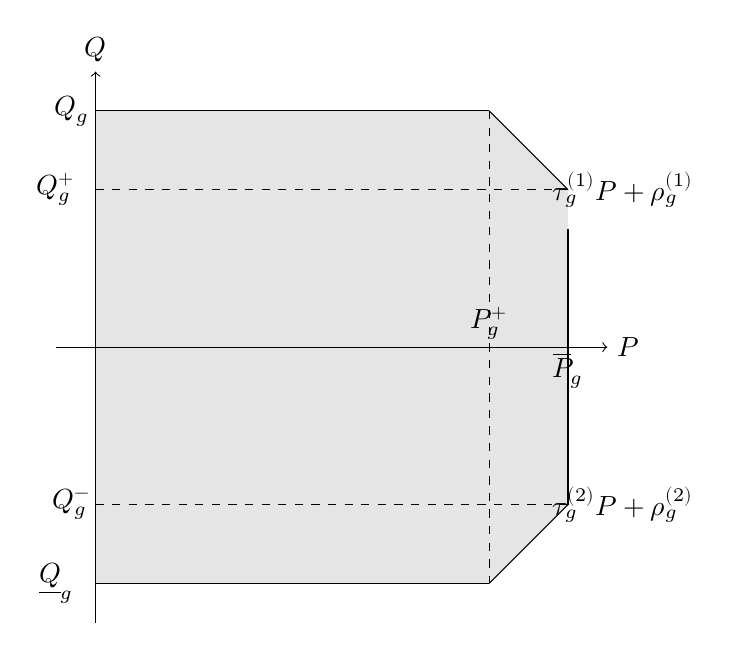
\begin{tikzpicture}

% Assi


% Area grigia
\fill[gray!20] (0,-3) rectangle (5,3);
\fill[gray!20] (5,-2) rectangle (6,2);
\fill[gray!20] (5,2) -- (6,2) -- (5,3) -- cycle;
\fill[gray!20] (5,-2) -- (6,-2) -- (5,-3) -- cycle;
% Linee tratteggiate orizzontali per Q
\draw (0,3) -- (5,3);
\draw[dashed] (0,2) -- (6,2);
\draw[dashed] (0,-2) -- (6,-2);
\draw (0,-3) -- (5,-3);

% Linee tratteggiate verticali per P
\draw[dashed] (5,3) -- (5,-3);

% Etichette per Q
\node at (-0.3,3) {$Q_g$};
\node at (-0.5,2) {$Q_g^+$};
\node at (-0.3,-2) {$Q_g⁻$};
\node at (-0.5,-3) {$\underline{Q}_g$};

% Etichette per P
\node at (5,0.3) {$P_g^+$};
\node at (6,-0.3) {$\overline{P}_g$};

% Linee inclinate e relative etichette
\draw (5,3) -- (6,2);
\draw (5,-3) -- (6,-2);

\draw (6,1.5) -- (6,-2);
\node at (6.7,2) {$\tau_g^{(1)} P + \rho_g^{(1)}$};
\node at (6.7,-2) {$\tau_g^{(2)} P + \rho_g^{(2)}$};

\draw[->] (-0.5,0) -- (6.5,0) node[right] {$P$};
\draw[->] (0,-3.5) -- (0,3.5) node[above] {$Q$};
\end{tikzpicture}
\end{center}

The problem could be stated in standard form as:

\[
\begin{aligned}
\min_{x \in \mathcal{D} \subseteq\mathbb{R}^2} \quad &\frac{1}{2}\|a - x\|^{2}_{2} \\
\textrm{s.t.}\quad & G x - h \leq 0\\
\end{aligned}
\]

with \(a = (a_P, a_Q)\), \(x = (P, Q)\) and:

\begin{equation}
G = \begin{pmatrix}
-1 & 1 & 1 & 0 & 0 & -\tau^{(1)}_g & \tau^{(2)}_g\\
0 & 0 & 0 & -1 & 1 & 1 & 1
\end{pmatrix}^T
\end{equation}

\begin{equation}
h = \begin{pmatrix}
-\underline{P}_g & \overline{P}_g & P^{\textrm{(max)}}_{g,t} & -\underline{Q}_g & \overline{Q}_g & \rho^{(1)}_g & -\rho^{(2)}_g
\end{pmatrix}^T
\end{equation}

With associated KKT conditions: \begin{align}
    G\hat{x} - h \leq 0&\\
    \lambda_i^* \geq 0& \quad i=1,\dots, 7\\
    G^T\hat\lambda = 0&\\
    (a-\hat{x}) + G^T\hat\lambda  = 0 &
\end{align}

\subsection{Experimental results}\label{experimental-results}

The problem described has a two-dimensional optimization variable, ten
scalar parameters and seven constraints:

\begin{equation}
 (X, \Lambda) = \mathrm{KINN}(\Theta)
\end{equation}

with: \begin{align}
\Theta \in \mathbb{R}^{N \times 10}, \quad&\Theta_{i} = (a_P^{(i)}, a_Q^{(i)},\overline{P}_g^{(i)}, \underline{P}_g^{(i)}, P_g^{+^{(i)}}, \overline{Q}_g^{(i)}, \underline{Q}_g^{(i)}, Q_g^{+^{(i)}}, Q_g^{-^{(i)}}, P^{\textrm{(max)}^{(i)}}_{g,t})\\
X \in \mathbb{R}^{N \times 2}, \quad&X_{i} = (P^{(i)}, Q^{(i)})\\
\Lambda \in \mathbb{R}_+^{0^{N \times 7}}, \quad&\Lambda_{i} = \lambda^{(i)}
\end{align}

At each training step, a random batch of parameters \(\Theta\) was
sampled:

\begin{align}
a_P^{(i)} &\sim U(0~\mathrm{p.u}., 1~\mathrm{p.u.})\\
a_Q^{(i)} &\sim U(-1~\mathrm{p.u}., 1~\mathrm{p.u.})\\
\overline{P}_g^{(i)} &\sim U(0.2~\mathrm{p.u}., 0.8~\mathrm{p.u.})\\
P_g^{+^{(i)}} &\sim U(0~\mathrm{p.u}., \overline{P}_g^{(i)})\\
\overline{Q}_g^{(i)} &\sim U(0.2~\mathrm{p.u}., 0.8~\mathrm{p.u.})\\
Q_g^{+^{(i)}} &\sim U(0~\mathrm{p.u}., \overline{Q}_g^{(i)})\\
P^{\textrm{(max)}^{(i)}}_{g,t} &\sim U(0~\mathrm{p.u}., \overline{P}_g^{(i)})
\end{align}

Models parameters were update to minimize the following loss function:

\[
\mathcal{L} = \frac{1}{N}\sum_{i=1}^N(\mathcal{L}_S^{(i)} + \mathcal{L}_{I}^{(i)}  + \mathcal{L}_{C}^{(i)})
\] where:

\begin{align}
    \mathcal{L}_S^{(i)} =& \|(a^{(i)}-\hat{x}^{(i)}) + G^{(i)^{T}}\hat\lambda^{(i)}\|_2\\ 
    \mathcal{L}_{I}^{(i)}  =& \|\max(0, G^{(i)}\hat{x} - h^{(i)})\|_2\\
    \mathcal{L}_{C}^{(i)}  =& \|G^{(i)^{T}}\hat\lambda^{(i)}\|_2\\
\end{align}

\subsubsection{Training}\label{training}

\begin{figure}

\centering{

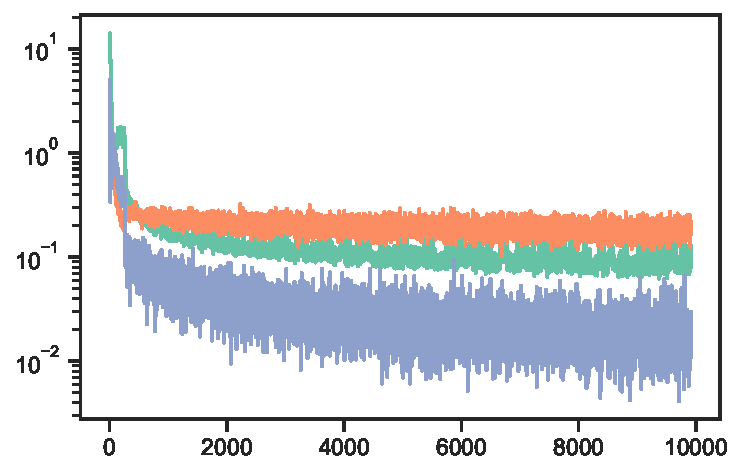
\includegraphics{Preprint_files/figure-pdf/fig-polar-output-1.pdf}

}

\caption{\label{fig-polar}A line plot on a polar axis}

\end{figure}%

\subsubsection{Evaluation}\label{evaluation}

\begin{figure}

\centering{

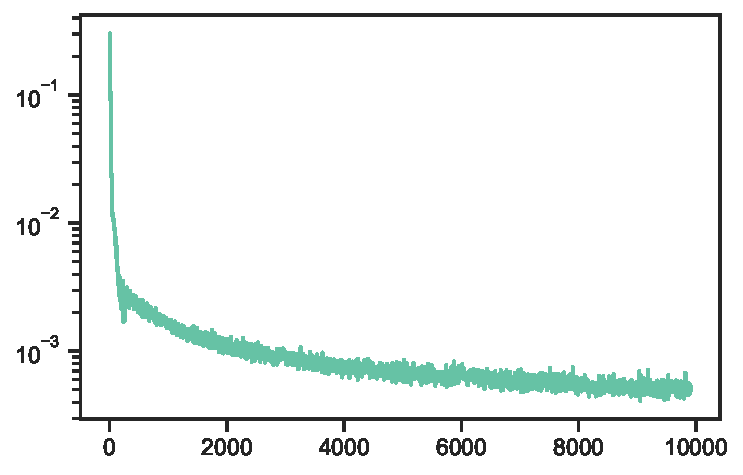
\includegraphics{Preprint_files/figure-pdf/fig-polar2-output-1.pdf}

}

\caption{\label{fig-polar2}A line plot on a polar axis}

\end{figure}%

\begin{figure}

\centering{

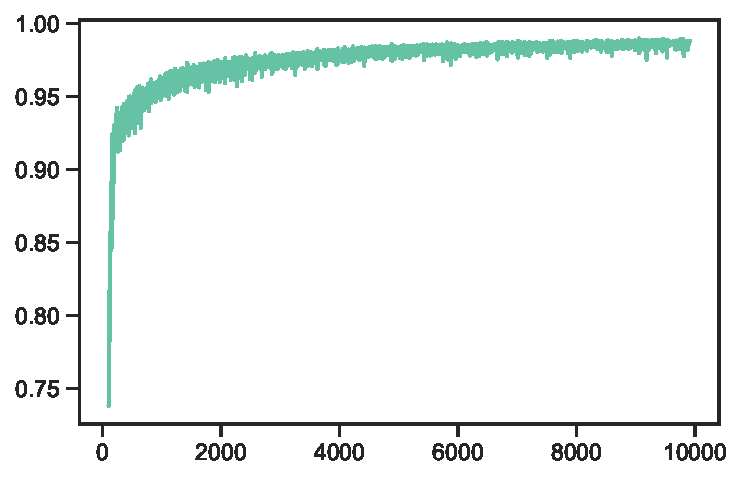
\includegraphics{Preprint_files/figure-pdf/fig-polar1-output-1.pdf}

}

\caption{\label{fig-polar1}A line plot on a polar axis}

\end{figure}%

\subsubsection{Comparison}\label{comparison}

\section{Conclusions}\label{conclusions}



\end{document}
